% ============================================================
% fig_architecture.tex  --  ROTP-PUF-FLASHER system overview
% Standalone TikZ source for fig_architecture.pdf
% Compile: pdflatex -interaction=nonstopmode fig_architecture.tex
% ============================================================
\documentclass[border=6pt]{standalone}
\usepackage[T1]{fontenc}
\usepackage{tikz}
\usetikzlibrary{positioning,arrows.meta,fit,backgrounds,calc}

\begin{document}
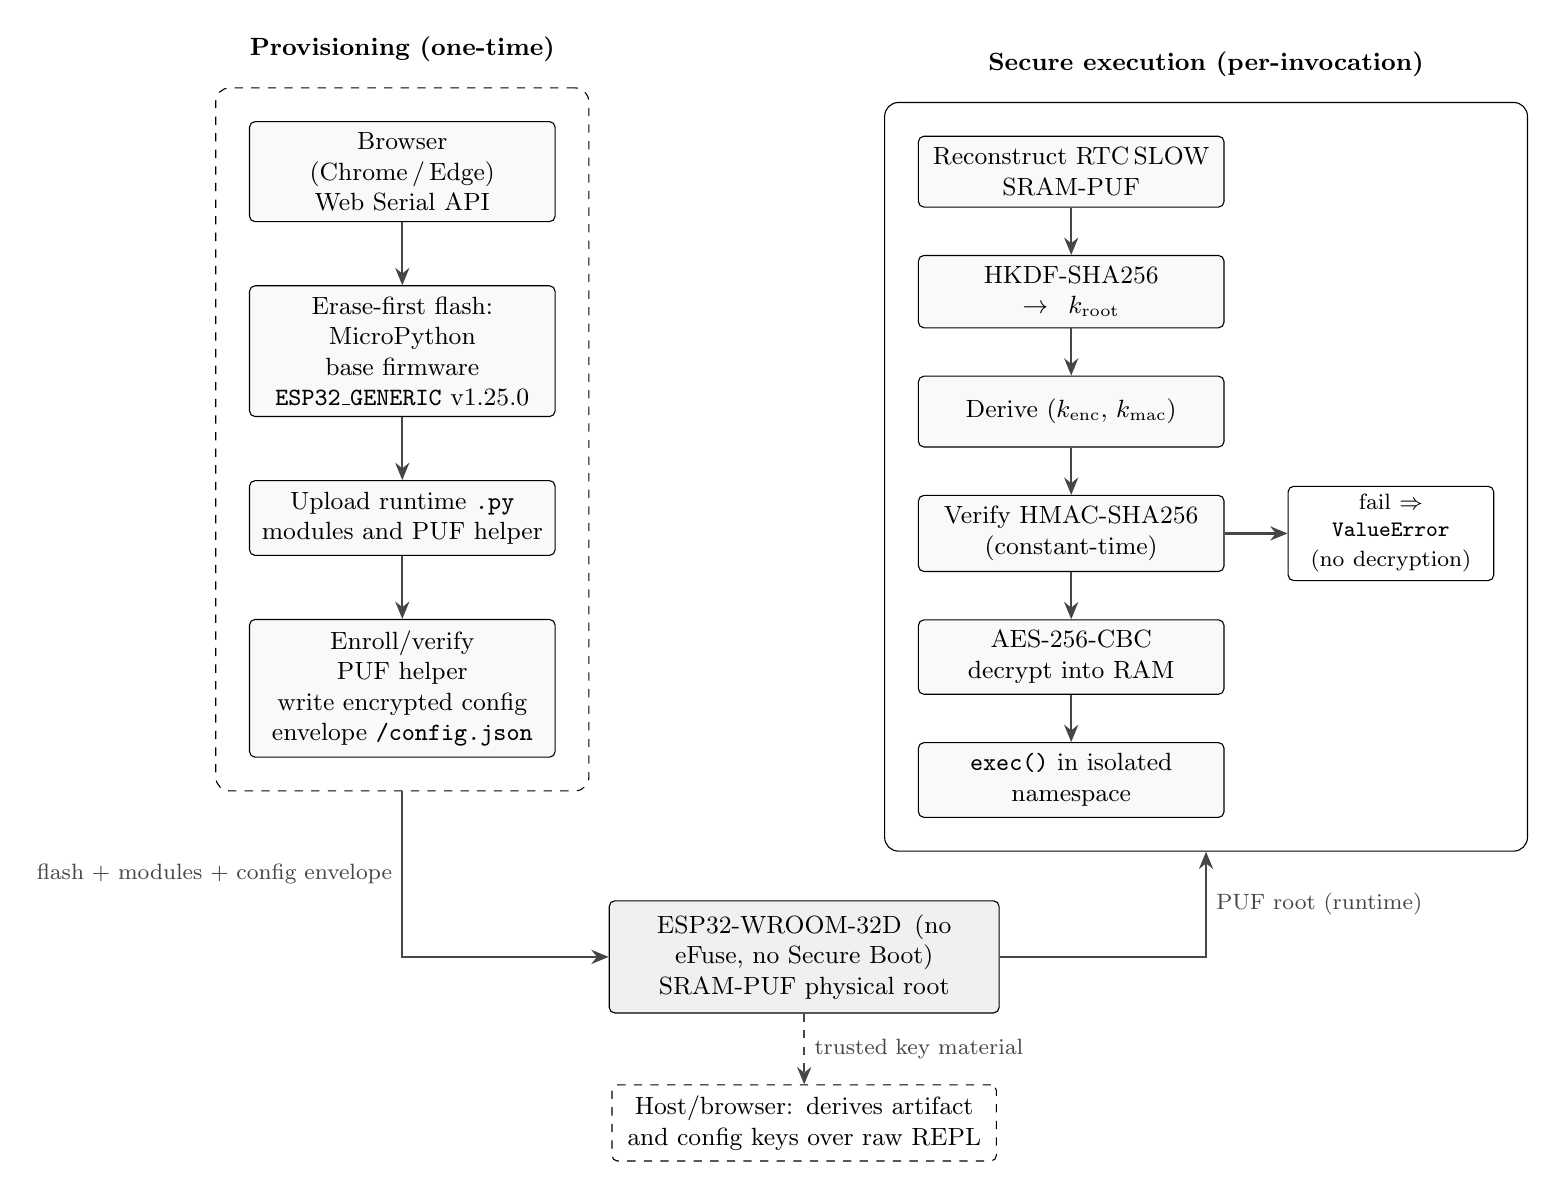
\begin{tikzpicture}[
  font=\small,
  >={Stealth[length=2.2mm,width=1.8mm]},
  box/.style={draw, rounded corners=2pt, align=center, inner sep=4pt,
              minimum height=9mm, fill=gray!5, text width=36mm},
  dev/.style={draw, rounded corners=2pt, align=center, inner sep=5pt,
              minimum height=9mm, fill=gray!12, text width=46mm},
  host/.style={draw, dashed, rounded corners=2pt, align=center, inner sep=4pt,
               fill=white, text width=46mm},
  failb/.style={draw, rounded corners=2pt, align=center, inner sep=3pt,
               fill=white, text width=24mm},
  phaseL/.style={draw, dashed, rounded corners=5pt, inner sep=12pt},
  phaseR/.style={draw, rounded corners=5pt, inner sep=12pt},
  arr/.style={->, thick, gray!55!black},
  arrx/.style={->, thick, dashed, gray!55!black},
]

% ---------- left column: provisioning (one-time) ----------
\node[box] (l1) {Browser (Chrome\,/\,Edge)\\Web Serial API};
\node[box, below=8mm of l1] (l2)
  {Erase-first flash:\\MicroPython base firmware\\\texttt{ESP32\_GENERIC} v1.25.0};
\node[box, below=8mm of l2] (l3)
  {Upload runtime \texttt{.py}\\modules and PUF helper};
\node[box, below=8mm of l3] (l4)
  {Enroll/verify PUF helper\\write encrypted config\\envelope \texttt{/config.json}};

\draw[arr] (l1) -- (l2);
\draw[arr] (l2) -- (l3);
\draw[arr] (l3) -- (l4);

% ---------- right column: secure execution (per-invocation) ----------
\node[box, right=46mm of l1] (r1) {Reconstruct RTC\,SLOW\\SRAM-PUF};
\node[box, below=6mm of r1] (r2) {HKDF-SHA256\\$\rightarrow k_{\mathrm{root}}$};
\node[box, below=6mm of r2] (r3) {Derive $(k_{\mathrm{enc}},\,k_{\mathrm{mac}})$};
\node[box, below=6mm of r3] (r4) {Verify HMAC-SHA256\\(constant-time)};
\node[box, below=6mm of r4] (r5) {AES-256-CBC\\decrypt into RAM};
\node[box, below=6mm of r5] (r6) {\texttt{exec()} in isolated\\namespace};

\draw[arr] (r1) -- (r2);
\draw[arr] (r2) -- (r3);
\draw[arr] (r3) -- (r4);
\draw[arr] (r4) -- (r5);
\draw[arr] (r5) -- (r6);
% fail-closed branch off HMAC verification
\node[failb, right=8mm of r4] (fail)
      {\footnotesize fail $\Rightarrow$ \texttt{ValueError}\\(no decryption)};
\draw[arr] (r4) -- (fail);

% ---------- phase containers (drawn before device/host) ----------
\begin{scope}[on background layer]
  \node[phaseL, fit=(l1)(l2)(l3)(l4)] (pL) {};
  \node[phaseR, fit=(r1)(r2)(r3)(r4)(r5)(r6)(fail)] (pR) {};
\end{scope}

% ---------- ESP32 device (shared physical root), centered below ----------
\coordinate (mid) at ($(pL.south)!0.5!(pR.south)$);
\node[dev, below=10mm of mid] (dev)
  {ESP32-WROOM-32D \,(no eFuse, no Secure Boot)\\SRAM-PUF physical root};

\draw[arr] (pL.south) |- (dev.west)
      node[pos=0.25, left, font=\footnotesize] {flash + modules + config envelope};
\draw[arr] (dev.east) -| (pR.south)
      node[pos=0.75, right, font=\footnotesize] {PUF root (runtime)};

% ---------- host (build time), below the device ----------
\node[host, below=9mm of dev] (host)
  {Host/browser: derives artifact\\and config keys over raw REPL};
\draw[arrx] (dev.south) -- (host.north)
      node[pos=0.5, right, font=\footnotesize] {trusted key material};

% ---------- phase titles ----------
\node[above=2mm of pL.north, font=\bfseries\small] {Provisioning (one-time)};
\node[above=2mm of pR.north, font=\bfseries\small] {Secure execution (per-invocation)};

\end{tikzpicture}
\end{document}
